\section*{Introduction}

Developed economies require the continuous flow of persons and goods in astounding volumes. This dependency justifies investment in the development and maintenance of a transportation sector which is, in its own right, economically significant. It is intuitive that the function of all transportation systems is to enable the actualization of latent activity. It follows that transportation systems should be assessed on that basis and that well designed systems are those which efficiently enable latent flows. Encompassing this paradigm is the field of transportation accessibility. Transportation accessibility is, in short, the study of the related phenomena of how structural and individual factors create latent flows and how transportation systems accommodate them. More efficient built environments minimize the edge traversal costs which exist between demand and supply nodes. More efficient transportation allows for individuals and businesses to access more opportunities for the same cost. In the long term, co-optimization of land-use and transportation is vital to maximizing accessibility.

Transportation accessibility is, inherently, a network problem. Any method which seeks to quantify accessibility must define the nodes and edges which comprise the region in question. In the modern world, all nodes are, to a greater or lesser extent, connected. Scoping an accessibility analysis can be highly determinative of outcome. Researchers and planners have primarily utilized the concept of transportation accessibility as it applies to routine household behavior and local travel \cite{Handy_2020}. From the personal transportation perspective, access is defined as the ease with which individuals can reach the opportunities they desire subject to land-use, transportation infrastructure, temporal availability, and individual preference. Land-use dynamics determine the distribution and demand for amenities such as jobs and services at different locations. Transportation systems determine the edge traversal costs such as travel time, effort, and price which impede flows \cite{Geurs_2004}. Temporal availability of opportunities and transportation modes restrict the utility of opportunities and transportation modes. Finally, individual characteristics such as age, income, and education predict attraction to opportunities  and transportation modes \cite{Miller_2018} effecting their utility.

The US and similar western nations are unusually car-centric by global standards \cite{PrietoCuriel_2024} for personal transportation. The access provided by a road transportation system for \glspl{bev} is different than that for \glspl{icev} due to vehicular and supply network characteristics. Modern \glspl{bev} possess sufficient practical ranges to accomplish much daily of daily travel as shown in Figure \ref{fig:utility_factors} with data from \cite{NHTS_2017, NHTS_2022}. However, for long itineraries \glspl{icev} offer greater accessibility compared to \glspl{bev} due to vehicle ranges and the extensive availability of fueling stations in contrast to DC charging stations. Fueling stations are widely distributed across urban, suburban, and rural areas, ensuring that drivers have convenient access to refueling points wherever they travel. In contrast, the  charging network is less developed and distributed. This infrastructure gap poses challenges for \gls{bev} drivers, especially in remote or less densely populated areas, leading to concerns about range anxiety and limitations on travel options. Inadequate long-trip accessibility for \gls{bev} may result in cancellations or mode switches, often favoring \gls{icev} or air travel.

\begin{figure}[H]
	\centering
	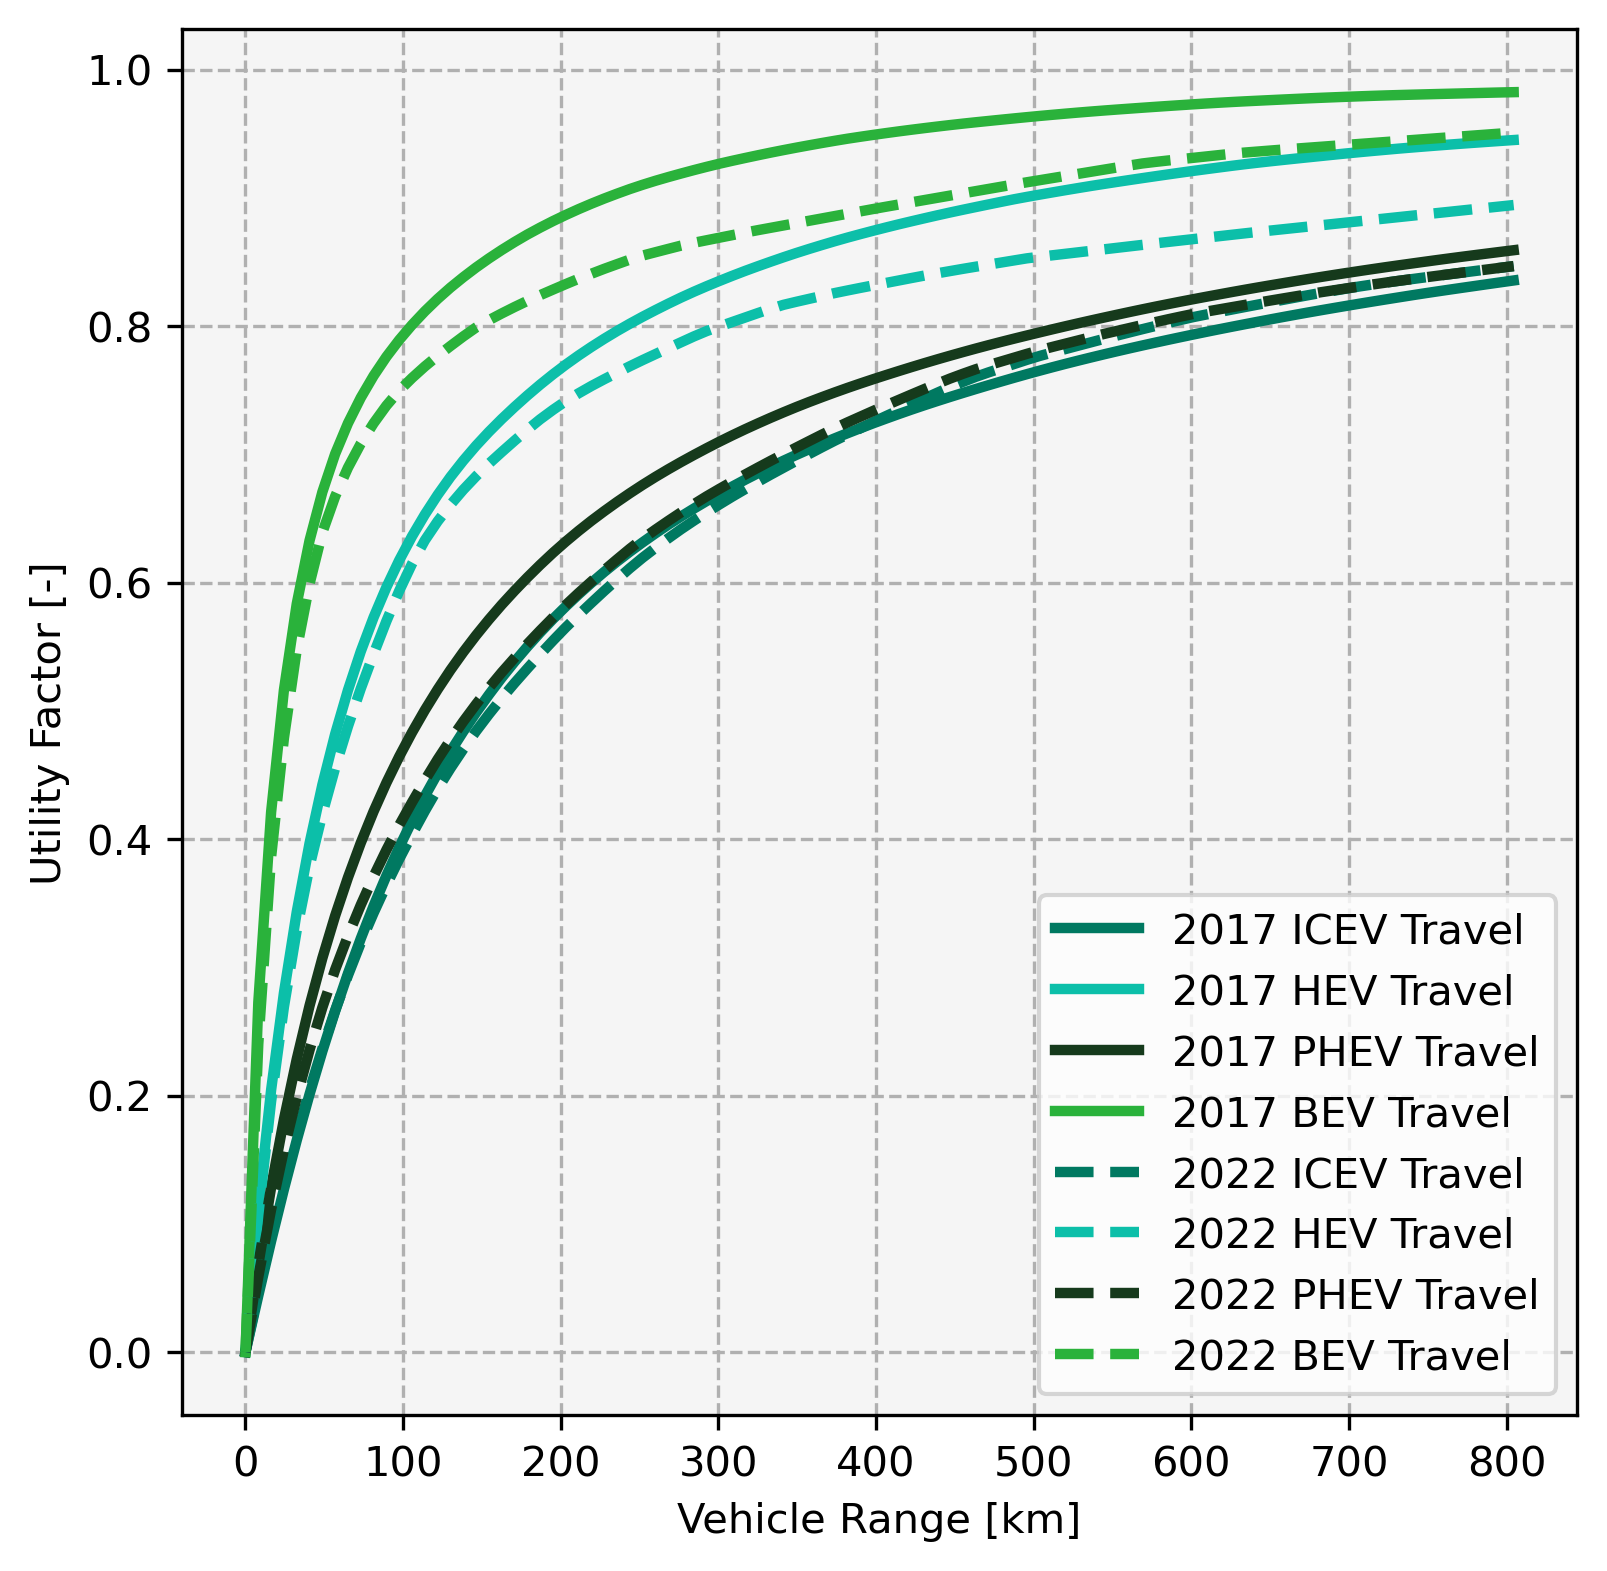
\includegraphics[width = \linewidth]{figs/UF_2017_2022_km.png}
	\caption{Individual vehicle routine travel utility factors as a function of range by powertrain type for \gls{nhts} 2017 and 2022 editions.}
	\label{fig:utility_factors}
\end{figure}

Disparities between the fueling and DC charging networks result from differences in their economic models. Gas pumping equipment requires lower up-front costs than DC \gls{evse}, is cheaper to operate \cite{Gamage_2023}, and has been deployed for far longer. Gas is often sold at low margin with stations making most profit on convenience items. Nearly all light-duty \gls{icev} drivers source all of their fuel from public fueling stations regardless of travel behavior. \gls{bev} drivers are expected to, and currently do, source much of their electricity from AC supply equipment during long dwells, often at private chargers \cite{Hardman_2018}. Thus DC charging stations are subject to higher capital expenditure, lower revenue potential, and less accumulated investment. To overcome these disadvantages, public investments in DC charging infrastructure must be made judiciously. Evaluation methods for potential charging stations should consider their network-wide impact on accessibility considering vehicle types, equipment reliability, and driver risk attitudes.

This study introduces a novel methodology to assess transportation accessibility for long vehicular trips. The methodology measures accessibility by computing optimal-feasible travel routes for \gls{od} pairs using a stochastic routing algorithm subject to vehicle range limitations, supply infrastructure, and driver risk attitudes. This methodology is powertrain agnostic and can be used to directly compare accessibility for vehicles with different ranges and which rely on different supply networks. Additionally, a case study is presented for the state of California showing a comparison between \glspl{icev} and \glspl{bev} access for important \gls{od} pairs within the state. The methodology introduced, as well as the open-source code provided in the supplemental information is a valuable tool for planners and policymakers in originating and evaluating \gls{evse} deployment policies.